% Repository:  https://github.com/chiehrosswang/TRB_LaTeX_tex
%
% Transportation Research Board conference paper template
% version 4.0 Lite (updates made to be compatible in Overleaf and ShareLaTeX)
%
%
% When numbered option is activated, lines are numbered.
\documentclass[numbered]{trbarticle}
\usepackage{graphicx}
\usepackage{booktabs}

\newread\somefile
\usepackage{xparse}

\usepackage{natbib}
\bibliographystyle{unsrtnat}
\setcitestyle{round}

% \usepackage[colorlinks=true,linkcolor=blue,citecolor=blue]{hyperref}
% For TRB version hide links
\usepackage[hidelinks]{hyperref}

% Put here what will go to headers as author
\AuthorHeaders{}
\title{Calibrating Ramp Meter Queue Length Models: Evidence from Utah}

% TODO: add macros for easier formatting of \author.
\author{%
    \textbf{Tanner Daines}\\
  \textit{}
  Graduate Student\\
  BYU\\
  \href{mailto:tdaines@byu.edu}{\nolinkurl{tdaines@byu.edu}}\\
  \hfill\break
    \textbf{Gregory Macfarlane}\\
  \textit{Corresponding Author\\}
  Assistant Professor\\
  BYU\\
  \href{mailto:gregmacfarlane@byu.edu}{\nolinkurl{gregmacfarlane@byu.edu}}\\
  \hfill\break
    \textbf{Grant Schultz}\\
  \textit{}
  Professor\\
  BYU\\
  \href{mailto:gschultz@byu.edu}{\nolinkurl{gschultz@byu.edu}}\\
  \hfill\break
  }

% If necessary modify the number of words per table or figure default is set to
% 250 words per table
% \WordsPerTable{250}

% If words are counted manually, put that number here. This does not include
% figures and tables. This can also be used to avoid problems with texcount
% program i.e. if one does not have it installed.
\TotalWords{6534}

\begin{document}
\maketitle


\section{Abstract}
This is where the abstract should go.
\hfill\break%
\hfill\break%
\noindent\textit{Keywords}:  Transportation, Travel Behavior,  
\newpage

\hypertarget{intro}{%
\section{Introduction}\label{intro}}

As traffic on freeways continues to rise, developing a reliable method to regulate the flow of vehicles onto the freeway has become increasingly important. A primary method that was first implemented in the 1960s is the ramp meter. A ramp meter is a traffic signal that is placed on the freeway on-ramp, designed to control the rate at which vehicles enter the freeway and therefore prevent it from exceeding capacity. Although ramp meters may improve freeway traffic conditions, they often generate a queue, causing vehicles to wait on the ramp prior to entering the freeway.

Research has previously been done to estimate the queue length at on-ramps to freeways, but most conclude that while certain methods improve queue size estimation, each possess flaws would prevent it from being widely implemented across many ramps without significant calibration. This paper aims to improve these previously developed methods, thus providing algorithms that more accurately report the expected queue length and wait time on any given on-ramp that utilizes ramp metering.

This project will focus on estimating the queue length on three on-ramps throughout Davis, Salt Lake, and Utah Counties. The ramps chosen for analysis are the northbound on-ramp to I-15 at Layton Parkway in Davis County, the southbound on-ramp at Bangerter Highway in Salt Lake County, and the southbound on-ramp at University Avenue in Utah County.

Two methods to estimate queue length are discussed in this paper, including a conservation model and a Kalman filter model. The Kalman filter model includes several variations to find a method that most accurately reflects field-observed queue lengths. Various components of the ramp such as the number of lanes, the ramp length, its traffic volume and occupancy, the metering rate, and the time of day will be considered. By understanding the impact of these characteristics on ramp operation and using data gathered on the ramp, the expected queue length and wait time for vehicles can be computed.

\hypertarget{literature}{%
\section{Literature}\label{literature}}

When freeway operations consistently deteriorate during peak hours, ramp meters are often implemented on the on-ramp, thus regulating the flow of vehicles entering the freeway. By controlling the flow of vehicles onto the freeway, motorists can travel in more favorable traffic conditions, which can reduce crashes, improve overall travel time, and lower emissions \citep{papageorgiou2002freeway}. Although conditions on the freeway may improve when ramp meters are implemented, this often leads to increased wait time on the on-ramp. Several ramp metering algorithms have been used in an attempt to find a balance between freeway and ramp operations, though much remains to be accomplished; many citizens contend that ramp meters cause more delay than they aim to prevent (Liu et al.~2012). For example, Minnesota implemented ramp meters in 1969, and in the fall of 2000---at the request of citizens in the Minneapolis-St.~Paul area---the meters were shut off for eight weeks to analyze whether freeway conditions were superior with the ramp meters (Levinson and Zhang 2004). To the surprise of some traffic analysts, some areas of the Twin Cities showed decreased travel time without the ramp meters, though the results mostly showed that travel delay, average speed, and travel time performed significantly better with the ramp meters in use. Other areas throughout both the United States and the world have shown similar results. In San Diego, a recently implemented ramp metering algorithm reduced travel time by more than four percent (Belisle et al.~2019). The Seattle Bottleneck algorithm, used in many locations, has also reduced crash rates and average travel time (Jacboson et al.~2006). Thus, in order to best understand the benefits of ramp meters, it is imperative that their function be established.

There are two primary classifications of ramp meters: pre-timed meters and traffic-responsive meters (Jacobson et al.~2006). Pre-timed meters operate at a set rate based on historical data; this type of metering has proven effective when traffic volumes are easily predictable. However, when sudden changes in traffic operations occur, pre-timed meters often fail to account for the change without manual intervention. Traffic-responsive metering on the other hand relies on real-time data collection through the use of loop detectors, which can be placed within the pavement or in the form of traffic cameras. Due to the extensive amount of data being collected, the initial calibration of traffic-responsive meters can prove to be time consuming; however, once effectively implemented, they can mitigate congestion based on the data received on the ramp.

By using loop detectors on the ramps, time occupancy and traffic volume data are gathered. Occupancy refers to the percent of time a point on the road is occupied by a vehicle; for example, if no vehicle passes over the detector during a given time period, the occupancy would be 0 percent, whereas if a vehicle was detected passing over the detector during half of that same time period, the time occupancy would show 50 percent. \citet{wu2009experiment} use the volume and occupancy data from the detectors by comparing three methods of calculating the queue length, including a Kalman filter, a conservation model, and the Highway Capacity Manual (HCM) back of queue method (the HCM method proved to be ineffective, and will not be discussed in detail in this literature review). The original equations developed for the conservation model and Kalman filter algorithms required the volume entering and exiting the ramp to be equal, but through analysis, they found that the detectors introduced error when compared with field recorded traffic volumes.

Many difficulties are introduced when relying solely on the detector data, particularly that vehicles can be double-counted or missed altogether (Wu et al.~2008). Because of this potential for error, the original conservation model equation and Kalman filter equation were modified to balance the volumes entering and exiting the ramp, which is shown by a volume-balancing ratio (C) in each equation. Equation 1 is the conservation model equation with the volume-balancing ratio included, and Equation 2 and Equation 3 are the equations used for the Kalman filter method with the volume-balancing ratio.

\hypertarget{add-in-equations-here}{%
\subsection{Add in equations here?}\label{add-in-equations-here}}

Using the volume-balancing ratio previously mentioned, it is presumed the conservation model and Kalman filter algorithms will produce more accurate queue length estimates, which can then be used to calculate the expected vehicle wait time. \citet{wu2009experiment} explain that the volume-balancing ratio may be set as a constant value or may be calculated in real time. Prior to incorporating this volume-balancing ratio, when \citet{wu2009experiment} utilized Equation 2 to find the queue length estimate based on the occupancy data, they found the correlation between the estimated queue length and the time occupancy to be only 0.63. This research also concluded that the relationship between volume data from the detector and the estimated number of vehicles is nonlinear, as the results gave a correlation coefficient of merely 0.18 between the two variables. Therefore, it is likely there are other factors outside the capability of this equation that affect the queue length such as detector error, driver distraction, poor weather, and traffic incidents.

However, in analyzing 20 data sets from ramp meters in Milwaukee, Wisconsin, \citet{wu2009experiment} found that the volume-balancing ratio improved both the Kalman filter and the conservation models considerably in nearly all cases, and in only a select few cases were slightly more errors introduced. These errors were found to occur in the Kalman filter models because when the volume-balancing ratio is close to 1 (the detector volume entering and exiting the ramp are nearly equal), the Kalman filter coefficient K is also close to zero, but the equation still adds queue length to the estimate from the coefficient K, which would introduce additional error. In contrast, when the volume-balancing ratio is not close to 1, the Kalman filter equation yield more reliable results than the conservation model. Overall, both the Kalman filter and conservation model, especially when using the volume-balancing ratio, provide generally accurate estimates of the actual queue length, which can then be used to predict the expected wait time on the freeway entrance ramp.

\hypertarget{methods}{%
\section{Methods}\label{methods}}

The following packages are used in this project in R.

\hypertarget{model}{%
\subsection{Model}\label{model}}

The Kalman filter model applied by \citet{horowitz} is as follows:

\begin{equation}
q_i = q_{i-1} + c_i + k (\hat{q}_i - q_{i-1})
  \label{eq:kalman}
\end{equation}

\hypertarget{data}{%
\subsection{Data}\label{data}}

Three on-ramps to I-15 throughout Davis, Salt Lake, and Utah counties were chosen for data collection and analysis. These ramps include the northbound on-ramp at Layton Parkway in Davis County, the southbound on-ramp at Bangerter Highway in Salt Lake County, and the southbound on-ramp at University Avenue in Utah County. Data were collected during several periods, including August and September 2020, April 2021, and July 2021. 19 days of data were collected at Layton Parkway, while 5 days of data were collected at Bangerter Highway and University Avenue. These ramps were metered only during the PM peak period, with metering taking place between 4:00 - 6:30 PM at Layton Parkway, 3:30 - 5:45 PM at Bangerter Highway, and 4:30 - 6:15 PM at University Avenue.

There are loop detectors located at three locations on each metered on-ramp to I-15, including at the excessive queue (EQ), which is located shortly after the entrance to each ramp, the intermediate queue (IQ), located roughly in the middle of the on-ramp, and the passage queue (PQ), located directly after the ramp meter signal. These detectors collect both volume and occupancy data and are recorded in 60-second increments. In addition, the variable ramp meter rate (in units of veh/hr) for each minute is included with the detector data. The detector data used in this paper were obtained through UDOT for each data collection period.

The data collected manually was also completed in 60-second increments during the metered period and includes the number of vehicles in each lane at the EQ detector, the queue length at the ramp meter signal, and the total number of other vehicles on the ramp that have not yet reached the queue. The ramp length and the number of lanes at the ramp meter signal were also recorded.

\hypertarget{time-stamp-inconsistency}{%
\subsection{Time Stamp Inconsistency}\label{time-stamp-inconsistency}}

While data were being collected and analyzed, it was discovered that there was a distinct discrepancy in queue length estimates between the field and detector data. For each ramp, the two forms of data appeared to have inconsistent time stamps, causing the data to be shifted from one another, thus significantly reducing the accuracy of the queue length estimates. To accommodate for this discrepancy, a function was created in R to shift the field data either forwards or backwards up to three minutes in either direction based on the minimum root-mean squared error (RMSE) between the total field and detector volumes measured at the EQ detector. Once the field data were shifted to best match the detector data, the two spreadsheets were joined together for ease of analysis.

\hypertarget{analysis-parameters}{%
\subsection{Analysis Parameters}\label{analysis-parameters}}

Several parameters were selected to compare the field and detector data for each 60-second increment, such as the average IQ and PQ occupancy on each ramp, the meter rate (in units of veh/min), traffic density (veh/mi/ln), and flow (veh/hr). These parameters were calculated based on the field and detector data.

\hypertarget{nested-data}{%
\subsection{Nested Data}\label{nested-data}}

The data were then nested into 30-minute bins to create an optimized K for 30-minute periods rather than a single optimized K for each day. To ensure that the data contained sufficient observations, a filter of requiring greater than or equal to 5 observations per period to be used for analysis.

\hypertarget{results}{%
\section{Results}\label{results}}

Some \emph{significant} applications are demonstrated in this chapter.

\begin{verbatim}
## Warning in file_diff_dbl(chr): NAs introduced by coercion
\end{verbatim}

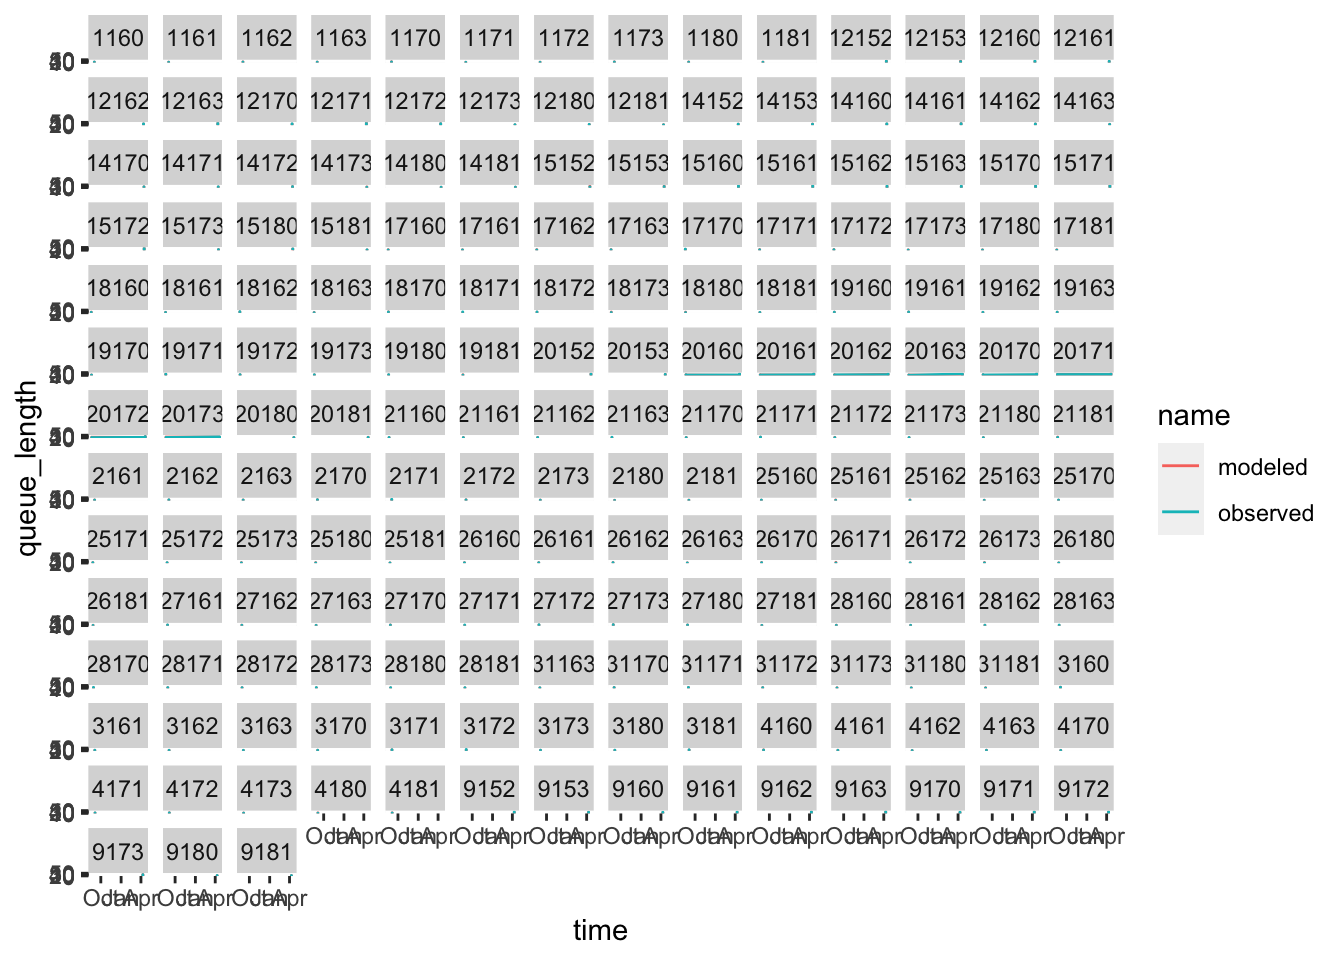
\includegraphics{ramp_meters_files/figure-latex/unnamed-chunk-1-1.pdf}

\hypertarget{linear-regression}{%
\subsection{Linear Regression}\label{linear-regression}}

\hypertarget{cluster-analysis-heuristics}{%
\subsection{Cluster Analysis / Heuristics}\label{cluster-analysis-heuristics}}

\hypertarget{final-words}{%
\section{Final Words}\label{final-words}}

We have finished a nice book.

\hypertarget{final-words-1}{%
\section{Final Words}\label{final-words-1}}

We have finished a nice book.

\hypertarget{acknowledgements}{%
\section*{Acknowledgements}\label{acknowledgements}}
\addcontentsline{toc}{section}{Acknowledgements}

This research was funded by the Utah Department of Transportation. The authors
alone are responsible for the preparation and accuracy of the information, data,
analysis, discussions, recommendations, and conclusions presented herein. The
contents do not necessarily reflect the views, opinions, endorsements, or
policies of the Utah Department of Transportation or the US Department of
Transportation. The Utah Department of Transportation makes no representation or
warranty of any kind, and assumes no liability therefore.

Cory Ward and James Umpress provided indispensible data prepration work.

\newpage
\bibliography{book.bib}


\end{document}
